\documentclass{article}
\usepackage[utf8]{inputenc}
\usepackage{fullpage}
\usepackage{amsfonts, amsmath, amsthm, amssymb}
\usepackage{tocloft}
\usepackage{maruth}
\usepackage{hyperref}
\usepackage{algorithm}
\usepackage{mdframed}
\usepackage{csquotes}
\usepackage{graphicx}
\usepackage[noend]{algpseudocode}
\usepackage{xcolor}
\hypersetup{
    colorlinks,
    linkcolor={red!50!black},
    citecolor={blue!50!black},
    urlcolor={blue!80!black}
}
\renewcommand{\O}{\mathcal{O}}
\renewcommand{\L}{\mathcal{L}}
\title{Foundations of ML and Data Science Notes}
\author{Maruth Goyal}
\date{Spring 2021}
\setcounter{tocdepth}{4}
\newtheorem{curse}{Curse}[section]
\newtheorem{theorem}{Theorem}[section]
\newtheorem{corollary}{Corollary}[theorem]
\newtheorem{lemma}{Lemma}[theorem]
\newtheorem*{remark}{Remark}
\newtheorem{defn}{Definition}[section]
\newtheorem{prop}{Property}[section]
\newtheorem*{example}{Example}
\newtheorem*{thm}{Theorem}

\newcommand{\lemmaautorefname}{Lemma}
\newcommand{\algorithmautorefname}{Algorithm}
\begin{document}

\maketitle
\tableofcontents
\section{Preface}
These notes are based very heavily on the lectures, and slides by Dr. Rachel Ward for the course CS395T: Foundations of Machine Learning and Data Science at The University of Texas at Austin from the Spring of 2021 (aka 2020 redux). Any errors introduced are mine. 
\section{Introduction}
\section{Linear Algebra Review}
\subsection{Matrix Norms}
\subsubsection{$p$-Norms}
\subsubsection{Frobenius Norm}
\subsubsection{Nuclear Norm}
\subsubsection{Entry-wise norms}
\subsection{Spectral Decomposition of Semi Positive Definite Matrices}
\subsection{Singular Value Decomposition}
\subsubsection{Principal Components Analysis}
\subsubsection{Power Method}
\subsubsection{QR Decomposition}
\section{Probability Review}
\subsection{The Gaussian Distribution}
\label{sec:prob:gaussian}
\subsection{$\chi^2$ Distribution}
\label{sec:prob:chi}
\subsection{Concentration Inequalities}
\label{sec:prob:conc}
\subsubsection{Markov's Inequality}
\label{sec:prob:conc:markov}
\subsubsection{Chebyshev's Inequality}
\label{sec:prob:conc:cheby}
% TODO: derivation, tightness
\subsubsection{Law of Large Numbers}
\label{sec:prob:conc:lol}
\subsubsection{Master Tail Bound}
\label{sec:prob:conc:master}
% TODO: Gaussian Annulus
% TODO: Expected length of Gaussian iid vectors
% TODO: Gaussian iid vectors orthogonal whp
\subsubsection{Chernoff Bounds}
\label{sec:prob:conc:chernoff}
\subsection{Sampling from Distributions}
\label{sec:prob:sampling}

\section{Geometry of High Dimensions}
\subsection{Properties of the Unit Ball}
\subsubsection{Surface Area of the Unit Ball}
\subsubsection{Volume of the Unit Ball}

\section{Curse and Blessings of High Dimensional Geometry}
\subsection{The Curse}
There are many well-studied ways of interpolating functions in low dimensions. For instance, linear interpolation, polynomial interpolation, spline interpolation, etc. from numerical analysis (see \autoref{sec:app:interp}). However, these methods break down in high dimensions. This is because of the {\em curse of dimensionality}.
\begin{curse}[Curse of Dimensionality]
The number of samples $f(x_j)$ needed to meaningfully approximate a function $f: [0,1]^d \to \R$ increases {\bf exponentially} in $d$.
\end{curse}
One way to see this is to see how many samples we would need to meaningfully approximate our domain. For instance, suppose our domain is the unit cube in $d$ dimensions, $[0,1]^d$. Let's say we want to approximate the domain by splitting it up into cubes of side $1/4$. i.e., we will divide the unit cube into cubes of side $1/4$ and then just sample one point from each of those cubes as a reasonably approximation of the unit cube. Well, that's still $\mathbf{4^d}$ points!
\begin{theorem}
Approximating the unit cube with samples from cubes of side $1/\epsilon$, requires $\O(\epsilon^d)$ samples. i.e., for any $\epsilon > 0$ we need to take $(1/\epsilon)^d$ samples $x_j \in [0,1]^d$ to form a grid resolution $\norm{{\mathbf{x}}_j - \mathbf{x}_k} = \epsilon$ with respect to any norm $\norm{\cdot} = \norm{\cdot}_p$.
\end{theorem}
Thus, in order to approximate functions in high-dimensions, we must be more clever. In particular, we need to exploit {\em strong additional information} about the function. Assumptions such as smoothness (i.e., existence of derivatives) are generally not strong enough.

\subsection{The Unit Ball}
As an example of how assumptions on our function might help us, we shall study functions which lie on the unit ball in $d$ dimensions. i.e., we have $f: \B^d \to \R$ where $\B^d = \set{x \in \R^d: \norm{x}_2^2 \leq 1}$. As cute and symmetrical as this domain seems, it has its own set of problems. For instance, observe that in $d$ dimensions there are $2^d$ orthants. Thus, even to just sample points on the surface of the ball in the direction of each of these orthants we need $2^d$ points, and even then we get a grid resolution of at most $\sqrt{2}$.

But what if we know something more about our function, and so can use fewer samples? How do we just generate samples from the unit ball?
    \subsubsection{Sampling from the Unit Ball}
    With computers, it is common and standard to have access to a psuedorandom generator (PRNG) which produces a stream of numbers indistinguishable to most common programs from a uniform distribution $\U[0,1)$. Thus, given access to a randomness oracle to sample from $\U[0,1]$, how do we sample from $\B^d$?
    \paragraph{Method 1: Sample from $[-1,1]^d$}
    One way to do this is to sample points from $\U[-1,1]^d$, and keep only those which are inside $\B^d$. This sounds great, and can be implemented in a single line of Python (though, what can't these days?), but there's an issue: in higher dimensions, we will end up keeping almost none of the points we sample. This happens because in high dimensions the ratio of the volume of the ball to the volume of the cube vanishes exponentially fast.
    
    \begin{theorem}[Volume of Unit Ball]
    The volume $V(d)$ of the unit ball $\B^d$ in $d$-dimensions is given as
    \begin{align*}
        V(d) = \frac{\pi^{d/2}}{\frac{d}{2}\Gamma\left(\frac{d}{2}\right)}
    \end{align*}
    \end{theorem}
    Observe that since $\Gamma\left(\frac{d}{2}\right) \sim \left(\frac{d}{2}\right)!$, we have that $V(d)$ decays exponentially in $d$. Moreover, the ratio of this volume to the unit ball would be given by
    \begin{align*}
        \frac{\pi^{d/2}}{\frac{d}{2}\Gamma\left(\frac{d}{2}\right)} \cdot 2^{-d}
    \end{align*}
    which decays at least as fast. Thus, for even relatively small $d$ this method becomes infeasible very quickly.
    \begin{curse}[Volume Ratios in High Dimensions]
    The volume of the unit sphere decays to $0$ exponentially fast in $d$. Moreover, the ratio of the volume of the unit sphere to that of the unit cube decays exponentially fast in $d$.
    \end{curse}
    Surely there is another way?
    
    \paragraph{Method 2: When in doubt, Gaussian}
    While the name of this paragraph is a bit of a giveaway, we shall nonetheless motivate why it's a good idea to call upon the mighty Gaussian. First, recall the density of the Gaussian (see \autoref{sec:prob:gaussian}:
    \begin{defn}[Gaussian Distribution]
    The univariate Gaussian distribution with mean $\mu$ and variance $\sigma^2$, written as $\N(\mu, \sigma^2)$, is defined as the distribution with density
    \begin{align*}
        p(x) = \frac{1}{\sqrt{2\pi \sigma^2}} \exp\left(\frac{-(x-\mu)^2}{2\sigma^2}\right)
    \end{align*}
    \end{defn}
    
    \begin{defn}[Multivariate Gaussian]
    The multivariate $d$-dimensional Gaussian distribution with mean $\mu \in \R^d$, and symnmetric positive semidefinite covariance matrix $\Sigma \in \R^{d \times d}$, written as $\N(\mu, \Sigma)$, is defined as the distribution with density
    \begin{align*}
        p(x) = \frac{1}{(2\pi)^{d/2} \sqrt{|\Sigma|}} \exp\left(-\half \cdot (x - \mu)^\top \Sigma^{-1} (x - \mu) \right)
    \end{align*}
    \end{defn}
    The key thing to observe is, if we look at the multivariate Gaussian $\N(\mathbf{0}, \mathbf{I})$ then the density becomes
    \begin{align*}
        p(x) = \frac{1}{(2\pi)^{d/2}} \exp\left(\frac{-(x_1^2 + x_2^2 + \dots + x_d^2)}{2}\right)
    \end{align*}
    That is, the distribution is {\bf spherically symmetric}. In other words, the density is the same for all vectors $x \in \R^d$ which lie on the surface of the same sphere. In particular, this means that sampling from this distribution amounts to sampling a random direction on the unit sphere (up to rescaling). You know what's even better? This is precisely the join density obtained by sampling $d$ i.i.d points from $\N(0,1)$.
    \begin{theorem}
    Sampling $\frac{x}{\norm{x}}$ where $\mathbf{x} \sim \N(0,1)^d$ is equivalent to sampling a point uniformly at random on the \textbf{surface} of the sphere.
    \end{theorem}
    Are we done? Nope! We can now generate points uniformly at random on the \textbf{surface} of the unit sphere, but we want to generate points uniformly at random \textbf{inside} the unit sphere. i.e., the surface and everything inside. Intuitively, once we have random points on the sphere, we should be able to simply rescale appropriately to get a point inside right? The answer is yes, but with some care.
    
    Suppose we simply sample a radius uniformly at random $r \sim \U[0,1]$ and rescale our point to be $r \cdot \frac{{\bf x}}{\norm{{\bf x}}}$. Does this work? Unfortunately, no. The reason is this way we will end up sampling \textbf{way} too many points close to the origin. Think about it this way: there are more points on the surface of the sphere of radius $1$ than the sphere of radius $0.1$. Thus, it makes sense to scale the probability of sampling a point at some radius with the number of points on the surface of the sphere of that radius. i.e., make it scale as the surface area of the sphere of radius $r$.
    
    \begin{theorem}
    In $d$ dimensions, the surface area of the sphere of radius $r$ is given by
    \begin{align*}
        S(r; d) = \frac{2\pi^{d/2}}{\Gamma\left(\frac{d}{2}\right)} \cdot r^{d-1}
    \end{align*}
    \end{theorem}
    Thus, we see that $S(r; d)$ scales as $r^{d-1}$. A quick integral shows that with appropriate normalization constants, the distribution we are looking for has density
    \begin{align*}
        p(r) = dr^{d-1}
    \end{align*}
    Thus we have the following final result:
    \begin{theorem}
    Sampling $r \cdot \frac{\mathbf{x}}{\norm{\mathbf{x}}}$ where $r \sim dr^{d-1}$ and $\mathbf{x} \sim \N(0,1)^d$ is equivalent to sampling a point uniformly at random from $\B^d$.
    \end{theorem}
    Note that we can sample from both $\N(0,1)$ and $dr^{d-1}$ with access to only $\U[0,1]$ (see \autoref{sec:prob:sampling}).
    
    \paragraph{A ``blessing'' of dimensionality}
    Until now we have mentioned multiple curses of high dimensionality. But surely it isn't all cursed? Well, if it's an reassurance one of the blessings of high dimensionality is that we ``know'' how random i.i.d vectors behave in high dimensions. In particular, recall the following from \autoref{sec:prob:conc:master}
    \begin{thm}
    For $X \sim \N({\bf 0}, {\bf I}_d)$ the expected length of $X$ is $\sqrt{d}$.
    \end{thm}
    \begin{proof}
    \begin{align*}
        \E\left[\norm{X}^2\right] = \E\left[\norm{X_1}^2 + \dots + \norm{{X_d}^2}\right] = d\E\left[\norm{X_1}^2\right] = d
    \end{align*}
    \end{proof}
    \begin{thm}[Gaussian Annulus Theorem]
    For a $d$-dimensional spherical Gaussian with unit variances, for any $\beta \leq \sqrt{d}$, all but at most $3\exp\left(-c\beta^2\right)$ of the probability mass lies within the annulus $\sqrt{d} - \beta \leq \norm{{\bf x}} \leq \sqrt{d} + \beta$, where $c > 0$ is a fixed positive constant.
    \end{thm}
    These two theorems put together tell us that in high dimensions, if we sample random Gaussian vectors, then with {\bf extremely} high probability these vectors will lie approximately on the sphere of radius $\sqrt{d}$. Thus, in high dimensions we have an increasingly confident sense of how these i.i.d Gaussian vectors behave.
\section{Random Projections, Johnson-Lindenstrauss Lemma}
    \subsection{Motivation: Approximate Nearest Neighbors}
        Suppose we are given a point, and want to classify it into one of, say, $10$
        different classes. If we already have a bunch of labeled data points $\D$,
        then intuitively one of the simpler ways to do this is to look at the point
        closest to the query point, and decide based on what class that point lies in.
        This is basically the nearest neighbors algorithm.
        \begin{defn}[Nearest Neighbors]
            Given a training set $\D = \set{(x_i, y_i)}_{i \in [n]}$, and a query point
            $q$, where $x_i, q \in \R^d$ and $y_i \in {\mathcal C}$, output
            \begin{align*}
                x_* = \argmin_{\x_j \in \D} \, \norm{\x_j - {\mathbf{q}}}_2
            \end{align*}
        \end{defn}

        However, observe that in order to compute the nearest neighbor of a point,
        we must compute $\O(n)$ distances, which takes $\O(nd)$ time for $d$-dim vectors.
        This very quickly becomes intractable as $n$, $d$ get even mildly large. Thus we
        may want to look for a suitable relaxation of the problem. Indeed, the simplest
        relaxation wherein instead of looking for the exact nearest neighbor we only ask for
        an $\epsilon$-approximate (multiplicative error) is a resonable choice. But then, how
        do we compute this efficiently?

        \subsubsection{Low Rank Approximations with SVD}
            You might think, well if dimension is the problem let's just reduce it!
            We know how to do that! Recall that we can utilize the SVD of a matrix
            to find the best rank $r$ approximation / subspace.

            If we do this, we will observe that the cost of projecting each query point
            into $r$ dimensional space is $\O(r \cdot d)$, and the cost of doing a
            nearest-neighbors search in $r$-dimensional space is $\O(n \cdot r)$,
            giving us a total run time of $\O((n + d) \cdot r)$. Great! We have
            successfully accomplished our mission, time to pack up our bags and-- not so fast(Of course, we cannot have nice things!).
            The issue with this method is, we have assumed that our query points lie in a subspace
            close to our training dataset. But what if it's an outlier which has negligible
            components in the subspace? Then any training example is a nearest neighbor,
            which is awful.
        
        \subsubsection{When in doubt, Gaussian}
            The title of this subsection is a theme which comes up extremely often. But yes,
            while SVD might have failed us, as we will see dear old Gauss has not. It turns out
            that if we pick a random $r$-dimensional subspace and project into it, then Euclidean
            distances are approximately preserved. Since with (approximate) nearest neighbors search
            we are only interested in the (ordering of) Euclidean distances this works perfectly.

            One way to project into these random subspaces is to consider an $d \times d$ orthogonal
            matrix, and then take only the first $r$ rows of it. Another way is to sample $r$ orthogonal
            unit vectors $u_1, \dots, u_r \in \R^d$, and then simply project onto the subspace induced
            by them. If, for instance, we sample from a standard Gaussian then you may recall that with
            high probability the vectors will be pairwise orthogonal.  Thus, we will define
            a random linear map $f: \R^d \to \R^r$ as the map given be $f(\x) = \lp \inn{u_1, \x}, \dots, \inn{u_r, \x} \rp$
            where each $u_i \sim \N(0, \I_d)$. Then, we get the following theorem:
            
            \begin{theorem}
            Let $\mathbf{v} \in \R^d$ be fixed, and $f: \R^d \to \R^r$ be a random Gaussian projection. Then, there
            exists a universal constant $c > 0$ such that for any $\epsilon \in (0,1)$
            \begin{align*}
                \Pr \lb \left| \norm{f(\mathbf{v})}_2 - \sqrt{r}\norm{\mathbf{v}}_2 \right| \geq \epsilon \sqrt{r} \norm{\mathbf{v}}_2 \rb \leq 3 \exp\lp -cr\epsilon^2 \rp
            \end{align*}
            \end{theorem}
            \begin{proof}[Proof Sketch]
                Assume $\norm{\mathbf{v}}_2$ is unit norm. Then $f(\mathbf{v})_i$ is i.i.d standard Gaussian, apply
                Gaussian Annulus theorem to finish.
            \end{proof}

            Thus we see that with high probability projecting into a
            random subspace preserves distances upto constant factors,
            which is all we need. Thus, we can now apply this to
            approximate nearest neighbors by fixing some $\epsilon > 0$
            and setting $r = \O(\frac{2\log{n}}{\epsilon})$.

            By the theorem, with probability at least $1 - \frac{1}{n^2}$
            we have $\norm{f(q) - f(\x_j)}_2 = (1 \pm \epsilon)\sqrt{r} \norm{q - \x_j}_2$.
            By union bound, with probability at least $1 - \frac{1}{n}$, this holds
            for all points in $\D$. Thus $$x_* = \argmin_{\x_j \in \D} \, \norm{f(\x_j) - f(q)}_2$$
            will be an $\epsilon$-nearest neighbor of $q$.
\section{Convex Functions}
\label{sec:convex}
% characterizations
% stationary points global minimizer
% strongly convex
% multivariate taylor theorem
% Lipschitz continuity of gradient equivalent to \grad^2 f(w) <= L \cdot I_{d \times d}

\section{Gradient Descent}
If you have spent more than an hour (or in some cases, a second) with someone involved in Computer Science (or increasingly, STEM in general) you have probably heard of gradient descent. The elevator pitch of the method is essentially ``start with a guess, and then move in the direction of steepest decrease''. Recall from multivariable calculus (or physics) that the negative gradient is the direction of steepest descent, hence the name. In this section we will first try to somewhat motivate the utility of gradient descent (as opposed to other optimization methods), and then take a gander at what it looks like in different settings. In particular, we will look at the various variants of GD, and analyze their performance in different settings.

\subsection{Least Squares problems}
\subsubsection{Motivation and Setup}
A simple way to build any sort of predictive model is to conjecture some form of a ``feature basis'', and then try to find the best fit of the data to this basis. For instance, we might want to find the best fit cubic polynomial, or combination of sine/cosine waves, or even just a best-fit linear model. In each case, it's a matter of finding the coefficients $\inn{c_1, \dots, c_k}$ which results in our resultant function's evaluation on the training points match the expected output.

More formally, we may define a matrix $\A \in \R^{n \times d}$ such that
\begin{align*}
    \A_{ij} = \varphi_i\left(x^{(j)}_i\right)
\end{align*}
where $\inn{\varphi_1, \dots, \varphi_d}$ defines our feature basis. Then, our task is to solve
\begin{align*}
    \A\bx = {\bf b}
\end{align*}
where $\bx$ is our vector of coefficients. We will generally consider the case where this system is overdetermined. i.e., where we have more training samples than coeffecients $(n > d)$. In a practical setting, it is more feasible to instead look for an approximate solution $\bx$ simply satisfying $\A\bx \approx {\bf b}$.

One way to do it is to find $\bx$ which minimizes some measure of ``badness''. We shall now refer to this measure as a ``loss function'', denoted as $\L$. Thus, we want to find
\begin{align*}
    \min_{\bx \in \R^d} \L(\A, \bx, {\bf b})
\end{align*}
It remains to determine what $\L$ is. Intuitively, $\L$ should certainly involve the error $\A\bx - {\bf b}$. We could pick
\begin{align*}
    \L(\A, \bx, {\bf b}) = \norm{\A\bx - {\bf b}}_0
\end{align*}
where $\norm{u}_0 = |\mathrm{supp}(u)|$ is the number of non-zero entries in a vector. Intuitively, this is trying to find the ``simplest'' solution, as a proxy for generalization (along the lines of Occam's razor). However, this is a combinatorially hard problem, and thus perhaps not a great idea. What about
\begin{align*}
    \L(\A, \bx, {\bf b}) = \norm{\A\bx - {\bf b}}_1
\end{align*}
Well, minimizing the $1$-norm is at some level a proxy for minimizing the $0$-norm so it's a good idea in that sense. However, it is not differentiable everywhere. Differentiability is in general a good property to have, as it makes the problem amenable to various optimization techniques. What about the $2$-norm?
\begin{align*}
    \L(\A, \bx, {\bf b}) = \norm{\A\bx - {\bf b}}_2^2
\end{align*}
You might have noticed I sneaked in a square in there. As it turns out, the $2$-norm is somehow the Goldilocks zone of norms (see Scott Aaronson's lecture notes on Quantum Information Science \cite{aaronson_2018} for a similar observation in that realm). This loss function is twice-differentiable everywhere, and {\em convex} (see \autoref{sec:convex}). As we will see soon, this means our problem has a unique solution, and moreover has a nice closed form.

    \subsubsection{Solving Least Squares}
        The problem we want to solve can now be written out as
        \begin{align*}
            \min_x \norm{\A\bx - {\bf b}}_2^2 = \min_x \sum_{i=1}^n \lp \inn{\A_{i, \bullet}, \bx} - b_i\rp^2 = \min_{x_1, \dots, x_d} \sum_{i =1}^n \lp \sum_{j = 1}^d \A_{ij}\bx_j - b_i \rp^2
        \end{align*}
        We let our loss function be $\L(x) = \half \norm{\A\bx - {\bf b}}_2^2$. Then, to minimize we solve for the stationary points of $\L$. However, since $\L$ is convex, this will also be the global minimizer!
        \begin{align*}
            \frac{\partial \L}{\partial \bx_j} = \frac{\partial}{\partial \bx_j} \half \sum_{i = 1}^n \lp \inn{\A_{i, \bullet}, \bx} - b_i \rp^2 
            = \sum_{i = 1}^n \lp \inn{\A_{i, \bullet}, \bx} - b_i \rp \frac{\partial}{\partial \bx_j} \lp \inn{\A_{i, \bullet}, \bx} - b_i \rp \\
            =  \sum_{i = 1}^n \A_{ij} \lp \inn{\A_{i, \bullet}, \bx} - b_i \rp = \inn{\lp \A_{1j}, \dots, \A_{nj} \rp, \A\bx - {\bf b}} \\ = \inn{\A_{\bullet, j}, \A\bx - {\bf b}}
        \end{align*}
        Thus, we have that the gradient $\grad \L$ satisfies
        \begin{equation}
        \label{eqn:leastsq:grad}
            \grad \L := \lp \frac{\partial \L}{\partial \bx_j}\rp_{j = 1}^d = \A^\top(\A\bx - {\bf b})
        \end{equation}
        Thus, solving for the stationary points,
        \begin{align*}
            \grad \L = 0 \\
            \iff \A^\top (\A\bx - {\bf b}) = 0 \iff \A^\top \A\bx = \A^\top {\bf b} \\
            \iff \boxed{\bx = (\A^\top \A)^{-1} \A^\top {\bf b}}
        \end{align*}
        The term $(\A \A^\top)^{-1}\A^\top$ is also known as the {\em Moore-Penrose psuedoinverse}.
        \begin{defn}[Moore-Penrose psuedoinverse]
        For a full-rank overdetermined matrix $\A \in \R^{n \times d}$, the matrix $\A^\dagger := (\A^\top \A)^{-1}\A^\top \in \R^{d \times n}$ is call the (Moore-Penrose) psuedoinverse of $\A$.
        \begin{enumerate}
            \item $\A^\dagger$ is a {\em left} inverse of $\A$. That is, $\A^\dagger \A = \I_{d \times d}$.
            \item The psuedoinverse $x^* = \A^\dagger$ is the solution to the linear least squares problem.
        \end{enumerate}
        \end{defn}
        \paragraph{Properties of the Psuedoinverse}
        The psuedoinverse also has the following interesting properties:
        \begin{prop}
        $\A\A^\dagger \in \R^{n \times n}$ is an {\rm orthogonal projection matrix} onto the subspace spanned by the columns of $\A$. Similarly $(\A\A^\dagger - \I)$ is an orthogonal projection onto the complementary space.
        \end{prop}
        \begin{prop}
        The vector $\A\bx^* = \A\A^\dagger {\bf b} \in \R^n$ minimizing the least squares loss is the projection of ${\bf b}$ onto the subspace $\A\A^\dagger$ spanned by the columns of $\A$.
        \end{prop}
        \subsubsection{Least Squares Example}
        A simple instance of least squares is finding the best linear fit to a data set. i.e., find the best line $mx + b$ minimizing the sum of squared {\em vertical} offsets
        \begin{align*}
            \min_{m,b} \sum_{i = 1}^n \lp mx_i + b - y_i\rp^2
        \end{align*}
        In matrix form,
        \begin{align*}
            \min_{m,b} \norm{\A \begin{pmatrix}m & b \end{pmatrix}^\top - {\bf y}}_2^2
        \end{align*}
        where
        \begin{align*}
            \A = \begin{pmatrix}
            x_1 & 1 \\
            x_2 & 1 \\
            \vdots & \\
            x_n & 1
            \end{pmatrix}
        \end{align*}
        The least squares solution can then be calculated as follows:
        \begin{align*}
            \begin{pmatrix}
                    m^* \\
                    b^*
            \end{pmatrix} = (\A^\top \A)^{-1} \A^\top {\bf y} \\
            m^* =
                    \frac{\sum_{i = 1}^n x_iy_i}{\sum_{i = 1}^n x_i^2} \quad  b^* = 
                    \frac{1}{n} \sum_{i = 1}^n y_i
        \end{align*}
        \subsubsection{Efficiency of Solving Least Squares}
        Solving the least squares problem using the above psuedoinverse method is quite inefficient, since just to compute a single vector $\bx^*$ we need to invert a large matrix which can be a very expensive operation. While it is true that as we saw above the unique solution $\bx^*$ can be obtained by solving the linear system
        \begin{align*}
            \A^\top \A \bx^* = \A^\top {\bf b}
        \end{align*}
        with highly specialized linear solvers, we are more interested in general iterative solvers that extend beyond simple linear models. This is where \textbf{gradient descent} comes in.
        
        \subsubsection{Solving Least Squares with Gradient Descent}
        Gradient Descent is an extremely general, and simple first-order optimization method. The key intuition/insight is that in order to minimize a function, we keep moving in the direction of the negative gradient. The reader may recall that this is the direction of steepest decrease.
        \begin{algorithm}[H]
        \label{algo:gd}
        \caption{Gradient Descent Psuedocode}
        \begin{algorithmic}[1]
        \Procedure{GradientDescent}{$f, \eta$}
        \State Initialize $x_0 \in_R \R^d$
        \While{not converged}
            \State $x_{t+1} = x_t - \eta \grad f(x_t)$
        \EndWhile
        \Return $x_{t+1}$
        \EndProcedure
        \end{algorithmic}
        \end{algorithm}
        Now, specifically for the case of linear least squares, we recall \autoref{eqn:leastsq:grad}
        \begin{align*}
            \grad \L = \A^\top (\A\bx - {\bf b})
        \end{align*}
        Thus, the least squares gradient descent update becomes
              \begin{algorithm}
        \label{algo:leastsq:gd}
        \caption{Linear Least Squares Gradient Descent}
        \begin{algorithmic}[1]
        \Procedure{LinearLeastSquaresGD}{$\A, {\bf b}, \eta$}
        \State Initialize $x_0 \in_R \R^d$
        \While{not converged}
            \State $x_{t+1} = x_t - \eta \A^\top (\A\bx - {\bf b})$
        \EndWhile
        \Return $x_{t+1}$
        \EndProcedure
        \end{algorithmic}
        \end{algorithm}
        
    \subsubsection{Convergence of Gradient Descent}
    Although we have this seemingly wonderful iterative algorithm, it is imperative that we also establish bounds on how long it will take for it to converge given some convergence criterion. If, for instance, it takes $\O(2^n)$ rounds, that's kind of useless. Well, thankfully as it turns out GD isn't useless, and in fact we can prove the following convergence guarantee:
\begin{mdframed}
    \begin{theorem}
        For the linear least squares problem, the gradient descent algorithm can meet the following convergence criterion in $\O(\log \epsilon)$ iterations, for any $\epsilon > 0$:
        \begin{align*}
            \norm{\bx_{t+1} - \bx^*}_2 \leq \epsilon \cdot \norm{\bx_0 - \bx^*}_2
        \end{align*}
    \end{theorem}
\end{mdframed}    

    \begin{proof}
    We will proceed by first bounding $\norm{\bx_{t + 1} - \bx^*}$, and then proving our choice of $\eta$ implies a convergence with the desired rate. Observe
\begin{align*}
    \bx_{t+1} - \bx^* = \lp \bx_t - \eta\A^\top(\A\bx_t - {\bf b}) \rp - \bx^* \tag{GD update}\\
    = \lp \bx_t - \eta \A^\top \lp \A\bx_t - \A\bx^* \rp \rp - \bx^* \tag{$\A\bx^* = {\bf b}$ by assumption}\\
    = \bx_t - \bx^* - \eta \A^\top\A \lp \bx_t - \bx^* \rp \\
    = (\I - \eta \A^\top \A)(\bx_t - \bx^*)
\end{align*}
We will now use the following property of the Frobenius norm
\begin{prop}
    The Frobenius norm $\norm{\cdot}_2$ on matrices is submultiplicative. i.e.,
    \begin{align*}
        \norm{\A {\bf B}}_2 \leq \norm{\A}_2 \norm{{\bf B}}_2
    \end{align*}
\end{prop}
Thus, we now obtain the following bound
\begin{align*}
    \norm{\bx_{t + 1} - \bx^*}_2 \leq \norm{\I - \eta \A^\top\A}_2 \cdot \norm{\bx_t - \bx^*}_2
\end{align*}
In order for convergence, we need this to be a decreasing series. In particular, we need $\norm{\I - \eta \A\A^\top}_2 < 1$. We now attempt to find $\eta$ so that this is satisfied.

We first make the following observation
\begin{lemma}
    For any matrix $\A \in \R^{n \times d}$, $\norm{\A}_2 \leq \sqrt{\min{(n, d)}} \cdot \lambda_{\max}(\A)$.
\end{lemma}
\begin{proof}
    \begin{align*}
        \norm{\A}_2 = \sqrt{\sum_{i=1}^{\min{(n,d)}} \sigma_i^2} \leq \sqrt{\min{(n,d)} \cdot \sigma_1^2} = \sqrt{\min{(n,d)}} \cdot \sigma_1
    \end{align*}
\end{proof}
Thus, we will now bound the largest eigenvalue of $(\I - \eta \A^\top\A)$ and then appropriately pick $\eta$ so we get a contraction. In particular, suppose $\A^\top \A$ has eigendecomposition $\A^\top\A = {\bf U} \Lambda {\bf U}^\top$. Then, $\I - \eta\A^\top\A$ has eigendecomposition ${\bf U} (\I - \eta\Lambda) {\bf U}^\top$ . In particular the eigenvalues satisfy
\begin{align*}
    1 - \eta\lambda_{\max} \leq \dots \leq 1 - \eta\lambda_{\min}
\end{align*}
Where $\lambda_{\min}, \lambda_{\max}$ are the smallest, and largest eigenvalues of $\A^\top\A$ respectively. Thus, since $n > d$, we have that $$\norm{\I - \eta \A^\top\A}_2 \leq \sqrt{d}(1 - \eta \lambda_{\min})$$. In order for this to be a contraction, we need
\begin{align*}
    \sqrt{d}(1 - \eta\lambda_{\min}) < 1 \\
    \iff \eta > \frac{1}{\lambda_{\min}}\lp 1 - \frac{1}{\sqrt{d}}\rp 
\end{align*}
Thus, in particular $\eta = \frac{1}{\lambda_{\min}}\lp 1 - \frac{1}{\alpha\sqrt{d}} \rp$ for some $\alpha > 1$ satisfies our requirement. However, we can get a tighter bound if we have the following:
\begin{align*}
    \lp 1 - \frac{1}{\sqrt{d}} \rp \leq \frac{\lambda_{\min}}{\lambda_{\max}} \\
    \iff \kappa(\A^\top \A) \leq \lp 1 - \frac{1}{\sqrt{d}} \rp^{-1}
\end{align*}
If this condition is satisfied, we can get away with $\eta = 1/\lambda_{\max}$. In either case, we get the following:
\begin{align*}
    \norm{\bx_{t+1} - \bx^*}_2 \leq \lp1 - \eta \lambda_{\min} \rp \cdot \sqrt{d} \cdot \norm{\bx_t - \bx^*}_2 \\
    \leq \lp \lp1 - \eta \lambda_{\min} \rp \cdot \sqrt{d}\rp^t \cdot \norm{\bx_0 - \bx^*}_2
\end{align*}
Thus we can meet the following convergence criterion for any $\epsilon > 0$ within $\O(\log \epsilon)$ iterations. The optimal rate is obtained when the aforementioned condition is satisfied, and we may pick $\eta = 1/\lambda_{\max}$.
\begin{align*}
    \norm{\bx_{t + 1} - \bx^*}_2 \leq \epsilon \cdot \norm{\bx_0 - \bx^*}_2
\end{align*}

    \end{proof}
    % \begin{corollary}
    %     For the linear least squares problem, the gradient descent algorithm has exponential convergence rate
    %       \begin{align*}
    %         \norm{\bx_{t+1} - \bx^*}_2 \leq \lp 1 - \frac{1}{\kappa(\A)} \rp^t \cdot \norm{\bx_0 - \bx^*}_2
    %     \end{align*}
    %     where
    %     \begin{align*}
    %         \kappa(\A) = \frac{\sigma_{\max}(\A)}{\sigma_{\min}(\A)}
    %     \end{align*}
    %     is the {\em condition number} of $\A \in \R^{n \times d}$, for $\eta = 1/\lambda_1$.
    % \end{corollary}
        
\subsection{Convergence of GD for Smooth Functions}
In Machine Learning in general, while model families come in different shapes and sizes -- from simple best-fit feature bases, to SVMs, to deep neural networks -- it is still a common occurence that the loss function $\L$ has a special property: smoothness.
\begin{defn}
A differnetiable function $f$ is called \textbf{smooth} iff it has a Lipschitz continuous gradient. i.e., there exists $L$ such that
\begin{align*}
    \norm{\grad f(y) - \grad f(x)}_2 \leq L \norm{y - x}_2
\end{align*}
\end{defn}
Thus, herein we shall equivalently assume that $\grad \L$ is $L$-Lipschitz for some $L$. To study the convergence of GD, we will attempt to bound $\norm{\grad \L(w_k)}^2$. In particular, we will show the following:
\begin{mdframed}
\begin{theorem}
Fix $\eta = 1/L$. Then, we will achieve stopping criterion $\norm{\grad \L(w_t)}^2 \leq \epsilon$ in at most
\begin{align*}
    t = \frac{2L[\L(w_0) - \L^*]}{\epsilon}
\end{align*}
where $\L$ is assumed to be smooth, and $L$ is the Lipschitz constant for $\grad \L$.
\end{theorem}
\end{mdframed}

In order to prove things about $\norm{\grad \L}^2$, it's a good idea to first get a bound for $\L(w)$ in terms of $\grad L$. We will utilize the following variant of the multivariate Taylor expansion:
\begin{theorem}
\label{thm:9:3}
For a $C^2$ function
\begin{align*}
    f(y) \leq f(x) + \grad f(x)^\top (y - x) + \half (y-x)^\top \grad^2f(x^*)(y - x)
\end{align*}
\end{theorem}
However, we also want to utilize our smoothness assumption on $\L$. We will make use of the following lemma:
\begin{lemma}
\label{lem:9:3:1}
For $C^2$ functions, Lipschitz continuity of the gradient is equivalent to
\begin{align*}
    \grad^2 f(w) \preccurlyeq L \cdot \I_{d\times d}
\end{align*}
    where $A \preccurlyeq B$ iff  $B - A$ is positive semidefinite. Equivalently, we have
    $v^\top \grad^2 f(w)v \leq L\norm{v}_2^2 \, \forall v,w$
\end{lemma}
We will now apply \autoref{lem:9:3:1} to \autoref{thm:9:3} to obtain the following ``Descent Lemma'':
\begin{lemma}[Descent Lemma]
For smooth $\L$, it is the case that
\begin{align*}
    \L(y) \leq \L(x) + \grad\L(x)^\top(y - x) + \frac{L}{2}\norm{y - x}^2
\end{align*}
\end{lemma}
The Descent Lemma also holds for $C^1$ functions. This lemma gives us a quadratic upper bound function for $f$, touching at $f(x)$. To get a sense of what kind of learning rate/step size we should use, it might be a good idea to look at the minimizer for this upper bound. A simple calculation shows that the minimizer is
\begin{align*}
    y - x - \frac{1}{L} \grad \L(x)
\end{align*}
i.e., one gradient step away from $x$, with learning rate $\frac{1}{L}$. Ok, so now we will pick a constant step-size $\alpha = 1/L$ as our starting point. Using this, we will be able to prove the following theorem:
\begin{mdframed}
\begin{theorem}
\label{gd:thm:smooth:convg}
Suppose that $\L$ is smooth, and we pick a step-size $\alpha = \frac{1}{L}$. Then, the following holds:
\begin{align*}
    \min_{k \in [t]}{\; \norm{\grad \L(w_k)}^2} \leq \frac{2[\L(w_0) - \L^*]}{t}
\end{align*}
\end{theorem}
\end{mdframed}

\begin{proof}
Suppose we pick $\alpha = 1/L$. Then, our gradient update is the following:
\begin{align*}
    w_{t+1} = w_t - \frac{1}{L}\grad \L(w_t)
\end{align*}
Substituting this into the ``Descent Lemma'' from \ref{lem:9:3:1} we get
\begin{align*}
    \L(w_{t+1}) \leq \L(w_t) + \grad \L(w_t)^\top \lp -\frac{1}{L} \cdot \grad \L(w_t)\rp + \frac{L}{2} \norm{\frac{1}{L} \grad \L(w_t)}^2 \\
    = \L(w_t) - \frac{1}{L}\norm{\grad\L(w_t)}^2 + \frac{1}{2L} \norm{\grad \L(w_t)}^2 \\
    = \L(w_t) - \frac{1}{2L}\norm{\grad \L(w_t)}^2 \\
    \L(w_{t+1}) \leq \L(w_t) - \frac{1}{2L}\norm{\grad\L(w_t)}^2
\end{align*}
We may rearrange this last result to get
\begin{align*}
    \norm{\grad \L(w_t)}^2 \leq 2L\left[\L(w_t) - \L(w_{t+1})\right]
\end{align*}
Finally, we sum up the squared norms of these gradients to get
\begin{align*}
    \sum_{k = 1}^t \norm{\grad L(w_t)}^2 \leq 2L \sum_{k = 1}^t\left[\L(w_k) - \L(w_{k+1})\right] 
    \leq 2L\left[\L(w_0) - \L(w_{t+1})\right] \leq 2L\left[\L(w_0) - \L^*\right]
\end{align*}
where $\L^*$ is the minimum value of $\L$. Thus, we derive our final result
\begin{align*}
        \min_{k \in [t]}{\; \norm{\grad \L(w_k)}^2} \leq \frac{2[\L(w_0) - \L^*]}{t}
\end{align*}

\paragraph{Picking $\alpha$ in practice}
It's not really a good idea to compute $L$ in order to use $\alpha = 1/L$ in practice, since computing $L$ is usually very expensive to compute. Moreover, this is a very small step-size as it is a \textbf{worst}-case bound on curvature. Generally, it is preferred to use line-search techniques.

For instance, we may decrease $\alpha$ by binary search until the following {\em Armijo condition} is met:
\begin{align*}
    f(w_t - \alpha\grad f(w_t)) \leq f(w_t) - \alpha\gamma\norm{\grad f(w_t)}^2  \quad \gamma \in (0, 1/2]
\end{align*}
\end{proof}

\subsubsection{Concluding Notes}
The cost of computing a gradient scales with the number of variables $d$. Thus, if we are working with $n$ training samples and computing a gradient, by linearity of the gradient it'll take us $\O(nd)$ time. Above, we showed that for smooth functions GD has a guaranteed $O(1/t)$ convergence rate. i.e., if we want to converge to an $\epsilon$-approximation of a stationary point, $O(1/\epsilon)$ iterations suffice. But then, including gradient computations that's at least $\O(nd/\epsilon)$ time (huge!). This, however, (thankfully?) is at least in part an artifact of this being a very loose bound. Gradient descent is {\bf much} faster in practice. However, this does not mean GD is finding {\bf global} minimizers efficiently -- $\NP$-hard functions still exist.

In order to find global optimums of non-convex smooth functions, the fastest possible algorithms require $\O(1/\epsilon^d)$ iterations in the worst case. Smoothness is too ``local'' or ``weak'' of a model to overcome the curse of dimensionality.
\begin{displayquote}
{\em ``The biggest open question in neural network theory over the past 15 years: how is it possible that gradient descent tends to converge to global minimizers of (highly nonlinear, highly nonconvex) neural network loss functions in practice, as if such optimization problems were not much more complex than linear regression? What is the underlying structure of neural networks as implemented in practice that allows us to overcome the curse of dimensionality?'' -- R. Ward}
\end{displayquote}
Convex functions, however, are able to overcome the curse. In particular, $\O(1/\epsilon)$ iterations of GD will do the trick of bringing us $\epsilon$-close to a {\bf global} optimum, since with a convex function a stationary point is a global minimizer. There are even algorithms which can achieve $\O(1/\sqrt{\epsilon})$.
\paragraph{Nesterov's accelerated gradient method}
This method achieves the aforementioned $\O(1/\sqrt{\epsilon}$ bound. Instead of a simple constant-sized step, this method uses the previous gradient as well. In particular, it makes the following update:
\begin{align*}
    w_{t+1} = v_t - \alpha \grad f\lp v_t \rp \\
    v_{t+1} = w_t + \beta_t\lp w_{t+1} - w_t \rp
\end{align*}
This method with $\alpha_t = 1/L$ and $\beta_t = \frac{t -1 }{t + 2}$ achieves an error of $\O(1/t^2)$ after $t$ iterations.

\subsection{Convergence of GD for Convex Functions, Polyak-Lojasiewic Inequality}
While smoothness alone may not have been enough to overcome the curse of high dimensionality, all hope is not lost. Notice that for some ``nice'' functions, for instance overdetermined linear regression, gradient descent has a much faster convergence rate. In particular, it converges {\bf expoenentially} fast. A general property underlying many such ``nice'' functions is the {\em Polyak-Lojasiewic (PL) Inequality}.
\begin{defn}[Polyak-Lojasiewic Inequality]
\label{gd:defn:pl}
A function $f: \R^d \to \R$ satisfies the PL inequality iff
\begin{align*}
    \half \norm{\grad f(w)}^2 \geq \mu \lp f(w) - f^* \rp
\end{align*}
\end{defn}
\begin{example}
For the least squares regression problem, $\mu = \lambda_{\min{}}(X^\top X)$, and
\begin{align*}
    \norm{X^\top (Xw - y)}^2 \geq \lambda_{\min{}}(X^\top X)\norm{Xw - y}^2
\end{align*}
\end{example}
\begin{figure}
    \centering
    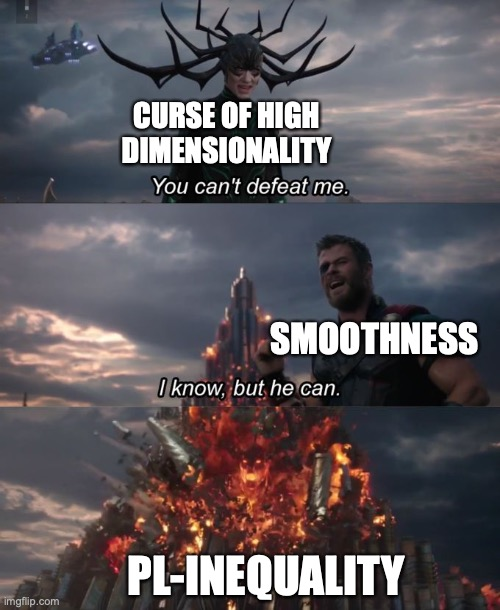
\includegraphics[scale=0.4]{50wuxh.jpg}
    \caption{A quality meme}
\end{figure}
\subsubsection{GD with Smooth Functions satisfying PL-inequality}
Now, using this PL-inequality, we will show that we can establish the following convergence rate:
\begin{mdframed}
\begin{theorem}
For a smooth function $f: \R^d \to \R$ which also satisfies the PL-inequality, for any $\epsilon > 0$ the following convergence criterion can be met in $\O(\log(1/\epsilon))$ iterations:
\begin{align*}
    f(w_t) - f^* \leq \epsilon
\end{align*}
\end{theorem}
\end{mdframed}

\begin{proof}
 Assuming smoothness of our function we were able to derive the following bound in the proof of \autoref{gd:thm:smooth:convg}
\begin{align*}
f \lp w_{t+1} \rp \leq f \lp w_t \rp - \frac{1}{2L} \norm{\grad f \lp w_t \rp }^2
\end{align*}
Under the PL-inequality (\autoref{gd:defn:pl}) we have
\begin{align*}
    -\norm{\grad f(w_t)}^2 \leq -2\mu \lp f(w_t) - f^*) \rp
\end{align*}
and thus,
\begin{align*}
    f(w_{t+1}) \leq f(w_t) - \frac{\mu}{L} \lp f(w_t) - f^* \rp \\
    f(w_{t+1}) - f^* \leq (f(w_t) - f^*) - \frac{\mu}{L} \lp f(w_t) - f^* \rp \\
    f(w_{t+1}) - f^* \leq \lp 1 - \frac{\mu}{L} \rp \lp f(w_t) - f^*) \rp \leq \lp 1 - \frac{\mu}{L}\rp^t (f(w_0) - f^*)
\end{align*}
Finally, observe that
\begin{align*}
    1 + x \leq e^x
\end{align*}
Thus
\begin{align*}
    f(w_{t+1}) - f^* \leq \exp\lp-\frac{\mu}{L} \cdot t\rp \left[f(w_0) - f^*\right]
\end{align*}
Hence, we have $f(w_t) - f^* \leq \epsilon$ for any $t$ satisfying
\begin{align*}
    t \geq \frac{L}{\mu} \log{(f(w_0) - f^*) / \epsilon)} = \O(\log(1/\epsilon))
\end{align*}
\end{proof}

\subsubsection{Properties of the PL-inequality}
The PL-inequality is general enough that it is satisfied by many standard convex models. However, it has the additional benefit of being satisfied even by some non-convex functions like $w^2 + 3\sin^2(w)$. It is also satisfied for many classes of {\em overparameterized} neural networks \cite{liu2020toward}, and is the reason for good empirical performance of GD in optimizing neural networks.

\subsubsection{Strong Convexity and PL-inequality}
Strong convexity, as the name may imply, is a stronger variant of convexity which induces some nice properties.
\begin{defn}[Strong Convexity]
A function is $\mu$-strongly convex if the following function is convex:
\begin{align*}
    f(w) - \frac{mu}{2}\norm{w}^2
\end{align*}

If $f$ is $C^2$, then equivalently
\begin{align*}
    \grad^2 f(w) \succcurlyeq \mu I
\end{align*}
\end{defn}
\begin{prop}
If $f: \R^d \to \R$ is a $\mu$-strongly convex function, then
\begin{enumerate}
    \item A {\em unique} minimizer exists
    \item if $f$ is additionally $C^1$, then it satisfies the PL inequality.
\end{enumerate}
\end{prop}
If we have a convex loss function $f$, then adding $\ell_2$-regularization makes it strongly convex. This can improve the convergence rate from $\O(1/t)$ to exponential. This motivates the weight-decay regularization technique used for neural networks.
\subsection{Stochastic Gradient Descent}
\section{Kernel Methods}
    \subsection{Linear Classification for Binary Data}
        Suppose we are given training data $\set{(x_i, y_i)}_{i \in [n]}$ where
        $x_j \in \R^d$ and $y_j \in \set{+1, -1}$. Suppose further that the data is
        linearly separable.

        \begin{defn}[Linearly Separable Data]
            A dataset is said to be linearly separable if there exists an {\bf affine} map
            $$\inn{{\bf w}, {\bf x}} - b$$ which separates the data. i.e.,
            $$ \hat{y_i} = {\rm sign}\lp \inn{{\bf w}, {\bf x}} - b \rp = y_j \quad \forall j $$
        \end{defn}
        Recall that $\w$ is a vector which is normal to the plane. ${\bf b}$ is roughly the intercept
        indicating how much the hyperplane is shifted in the direction of the normal $\w$. For instance,
        $\inn{e_1, \x} = b$ in $\R^3$ is simply the $y-z$ plane shifted $b$ in the $\x$-direction.
        The goal is to have all data points in one class to be on one side, and the others on the other. For linearly
        separable data, a ``best'' lienar classifier is often the one which {\em maximizes the margin}.
        i.e., maximizes the minimial distance between any point ${\bf x}_j$ and the hyperplane $\inn{{\bf w}, {\bf x}} - b$.
        Chosing the max-margin classifier is a good heuristic for generalization.

        For linearly separable data, there exist two parallel hyperplanes
        \begin{align*}
            \inn{\w, \x} - b = 1 \\
            \inn{\w, \x} - b = -1
        \end{align*}
        such that
        \begin{align*}
            \inn{\w, \x}_j - b \geq 1 \quad y_j = 1 \\
            \inn{\w, \x_j} -b \leq -1 \quad y_j = -1
        \end{align*}

        Thus, we want to maximize the distance between these two parallel
        hyperplanes subject to these constraints. We define the distance from a point $u$ to the hyperplane
        $H = \set{\x: \inn{\w, \x} = b}$ as 
        \begin{align*}
            d({\bf u}, H) = \min_x \, \norm{{\bf u} - \x}_2 \quad \text{s.t.} \  \inn{\w, \x} = b
        \end{align*}
        We will minimize this by the method of Lagrange multipliers. In particular, we define
        \begin{align*}
            d'(x; u) = \half \norm{x-u}_2^2 \quad \grad d'(x; u) = \x - {\bf u} \\
            \grad \inn{\w, \x} = \w \\
        \end{align*}
        Thus we must simply solve
        \begin{align*}
            \x - {\bf u} - \lambda \w = 0 \\
            \inn{\w, \x} = b
        \end{align*}
        Setting $x = {\bf u} + \lambda \w$ and substituting into the second equation we get
        \begin{align*}
            \inn{\w, {\bf u} + \lambda \w} = \inn{\w, {\bf u}} + \lambda \norm{w}_2^2 = b \\
            \implies \lambda = \frac{b - \inn{\w, {\bf u}}}{\norm{\w}_2^2}
        \end{align*}
        Finally, substituting back we obtain
        \begin{align*}
            \x = {\bf u} + \frac{b - \inn{\w, {\bf u}}}{\norm{\w}_2} \hat{w} \quad d(u, H) = \frac{b - \inn{\w, {\bf u}}}{\norm{\w}_2}
        \end{align*}
        Picking $\u = \lp 0, 0, \dots, 0, \frac{1 + b}{\w_d} \rp$ on the line $\inn{\w,\x} - b = 1$ we get
        $d(\u, H) = \frac{1}{\norm{\w}_2}$
        Thus, the distance between these two parallel hyperplanes is $\frac{2}{\norm{\w}_2}$. Maximizing
        this quantity is equivalent to minimizing $\norm{\w}^2_2$, which is a nice convex optimization
        problem. 

        \subsubsection{Support Vector Machine (SVM) Classification}
        If we look at the above constraints, and multiply both sides by $y_i$, then
        we may observe that we get the following optimization problem:
        \begin{align*}
            \min_{\w, b} \, \norm{\w}_2^2 \\
            \text{s.t.} \quad y_j \cdot \lp \inn{\w, \x_j} - b \rp \geq 1
        \end{align*}
        This is the Support Vector Machine (SVM) classification problem, developed at AT\&T Bell Labs by Vapnik et al. \cite{boser1992training} in the 1990s.
        They became famous at the time for beating neural networks with hand-designed features on handwriting recognition on the MNIST dataset.

        \begin{prop}
            Unlike neural networks, SVM is highly robust to outlier data points.
        \end{prop}
        Optimizing an SVM is really solving a constrained {\em Quadratic Program} (QP)
        \begin{defn}
            A quadratic program optimizing over some parameter $\z$ is defined as
            \begin{align*}
                \max_\z{} \; \half \z^\top \A \z - {\bf d}^\top \z \\
                \text{s.t.} \quad {\bf B}\z \leq e
            \end{align*}
        \end{defn}
        Now, the quadratic program stated above is in ``primal'' form. However, similar to linear programming, in quadratic
        programming it is easier to solve the ``dual'' program. In particular, for SVM the dual program is
        \begin{align*}
            \max_{\alpha \in \R^n}{} \lp \sum_{i= 1}^n \alpha_i \rp - \half \sum_{(i,j) \in [n] \times [n]} (y_i y_j) \cdot (\alpha_i \alpha_j) \cdot \inn{\x_i, \x_j}  \label{eqn:svm:dual} \\
            \text{s.t.} \quad \alpha_i \geq 0 \ \text{and} \ \sum_{i = 1}^n y_i \alpha_i = 0
        \end{align*}
        If $\alpha \in \R^n$ is the solution to this program, then the solution to the primal program $\w$ can be written as
        \begin{align*}
            \w = \sum (\alpha_i y_i) \cdot \x_i
        \end{align*}
        Important to note that $\alpha_i > 0$ when $\x_i$ lies on the boundary, or when it's a {\em support vector}. 

        % TODO: using SVM for N classes
        % TODO: soft-margin SVM for non-really-linearly separable    
\subsection{Kernel Trick for Non-Linearly Separable Data}
Often in real-world problems, data is structured, and separable, but perhaps not necessarily
linearly separable. When this situation arises, of course we cannot directly apply something like SVM
to it. However, we may apply a {\em kernel trick} by {\em lifting} our data to a higher dimension wherein
it does exhibit linear separability and apply SVM in the higher dimension. The linear boundary in the higher
dimension may correspond to a very non-linear seperator in the normal dimension.

\begin{defn}
    A kernel $K: \R^d \times \R^d \to \R$ can be any legal definition of an inner product
    \begin{align*}
        K(\x, \z) := \inn{\varphi(\x), \varphi(\z)} \quad \varphi: \R^d \to \R^D \; D >> d
    \end{align*}
\end{defn}

\begin{defn}[Kernel Trick]
    The idea of the kernel trick is the following:
    \begin{enumerate}
        \item Rewrite the algorithm (if possible) such that it only uses the data points $\x_i$ in the form of inner
        products $\inn{\x_i, \x_j}$
        \item Replace all inner products $\inn{\x_i, \x_j}$ with kernels $K(\x_i, \x_j)$
    \end{enumerate}
\end{defn}

\begin{example}[Polynomial Kernel]
    An intuitive example of a kernel is the polynomial kernel
    \begin{align*}
        K_r(\x, \z) := \lp \inn{\x, \z} \rp^r
    \end{align*}
    For $r = 2, d=2$
    \begin{align*}
        \varphi: \R^2 \to \R^3 : (x_1, x_2) \to \varphi(\x) = (x_1^2, x_2^2, \sqrt{2}x_1x_2)
    \end{align*}
    For the polynomial kernel of degree $r$, $K_r(\x, \z)$ lifts into a dimension which
    grows at least exponentially in $r$. However, since we are never explicitly computing $\varphi$,
    we just need to compute $r$ multiplications.
\end{example}
While the above Polynomial kernel is a nice toy example, it is not really used in practice. Instead, it is common
to use kernels such as the {\rm Gaussian} kernel which is an inner product in an infinite-dimensional space.
\begin{defn}[Gaussian Kernel]
    The Gaussian Kernel is defined as
    \begin{align*}
        K(\x, \z) = \exp \lp -\frac{\norm{\x - \z}_2^2}{2\sigma^2} \rp
    \end{align*}
\end{defn}
Since the Gaussian kernel operates in a ``radial basis'', it is able to provide linear separators for almost any data set.
However, it often separates way too well and thus overfitting.
There is also the $\tanh$ kernel, which when used with an SVM corresponds exactly to a $2$-layer neural-network.
\begin{defn}[$\tanh$ Kernel]
    The $\tanh$ kernel is defined as:
    $$K(\x, \z) = \tanh\lp \alpha \x^\top \z + c \rp$$
\end{defn}

\subsubsection{Kernel SVM and other Generalizations}
    Observe that the dual program for SVM is formulated in terms of just the inner products of the data points, $\inn{\x_i, \x_j}$. Thus,
    we may apply the kernel trick, resulting in the ``kernel SVM'' program:
    \begin{defn}[Kernel SVM]
        The generalization of SVM substituting kernels for inner products is defined by the parameters obtained from the following program
        \begin{align*}
            \max_{\alpha \in \R^n} \lp \sum_{i= 1}^n \alpha_i \rp - \half \sum_{(i,j) \in [n] \times [n]} (y_i y_j) \cdot (\alpha_i \alpha_j) \cdot k(\x_i, \x_j) \\
            \text{s.t.} \quad \alpha_i \geq 0 \ \text{and} \ \sum_{i = 1}^n y_i \alpha_i = 0
        \end{align*}
    \end{defn}
    
    As mentioned earlier this can let us find separating hyperplanes for non linearly seperable data by mapping into higher dimensions.
    However, for certain choices of Kernels the model becomes prone to overfitting. Thus, it is advisable to add a regularization term
    to prevent this. We may even want to explicitly allow some misclassification as a proxy for generalization. This results in the following
    general SVM formulation:
    \begin{defn}[Generalized SVM]
        The variant of SVM allowing for some classification error for each example, $\xi_j$, and a regularization parameter $\lambda$ upon $\w$
        is described by the following program:
        \begin{align*}
            \min_{\w, b,\xi} \  \lambda \norm{\w}_2^2 + \frac{1}{n} \sum_{j = 1}^n \xi_j \\
            \text{s.t.} \  y_i \cdot \lp \inn{\w, \x_j} - b\rp \geq 1 - \xi_j, \  \xi_j \geq 0, \  \forall j
        \end{align*}
    \end{defn}
    
\section{Appendix}
\subsection{Math Glossary for lowly CS majors}
\begin{defn}[Orthogonal Projection Matrix]
A matrix $\A \in \R^{n \times n}$ is an orthogonal projection matrix if $\A^2 = \A$ and $\A^\top = \A$.
\end{defn}
\begin{defn}[Gamma Function]
The Gamma Function $\Gamma(x): \R \to \R$ is defined as
\begin{align*}
    \Gamma(x) = \int_0^\infty t^{x-1}e^{-t} {\rm d}t
\end{align*}
Importantly, it satisfies $\Gamma(x) = (x-1)!$ for $x \in \Z^+$. In general, it satisfies $\Gamma(x) = x \cdot \Gamma(x-1)$.
\end{defn}
\begin{defn}[Hyperplane]
In $d$ dimensions, a hyperplane is a subspace of dimension $d-1$.
\end{defn}
\begin{defn}[Half-space]
A half space is either of the two parts that a hyperplane divides a space into.
\end{defn}
\begin{example}[half-space]
In $2$ dimensions, consider any line in the plane. Then the parts on either side of the line define half-spaces.
\end{example}
\begin{defn}[Orthant]
An orthant in $d$ dimensions is defined to be the intersection of $d$ mutually orthogonal half-spaces. The halfspaces induced by the standard bases for $\R^d$ induce $2^d$ orthants (for $d=2$, quadrants).
\end{defn}
\begin{example}[Orthants]
The upper right quadrant in $2$ dimensions is the intersection of the half-spaces $\set{(x,y) \in \R^2 \mid x \geq 0 }$ and $\set{(x,y) \in \R^2 \mid y \geq 0}$. 
\end{example}
\begin{defn}[Smoothness]
A function $f: A \to B$ is said to be smooth if it is infinitely-differentiable everywhere.
\end{defn}
\begin{defn}[Latent]
A variable which is inferred, but not observed is considered to be a latent variable.
\end{defn}
\begin{example}[Latent Variable]
Properties such as time taken to add to cart, time taken to check out cart, hit rate of recommendations etc are all measurable, but ``consumer satisfaction'' scores are inferred from these, not observed.
\end{example}
\subsection{Classical Interpolation Methods}
\label{sec:app:interp}
\subsubsection{Linear Interpolation}
\subsubsection{Polynomial Interpolation}
\subsubsection{Spine Interpolation}

\section{References}
\bibliographystyle{apalike}
\bibliography{references}
\end{document}
